\documentclass[PianoDiProgetto.tex]{subfiles}

\begin{document}

\chapter{Pianificazione}

\section{Analisi}
Il periodo di analisi comincia il 23-11-2017 e si conclude il 16-01-2018: l'inizio coincide con la formazione del gruppo e l'avviamento del lavoro; la conclusione con la scadenza scelta per la consegna dei documenti per l'entrata nel progetto. Durante questo periodo le attività principali svolte sono:
\begin{itemize}
	\item \textbf{Norme di Progetto:} questa attività consiste nella redazione delle \textit{Norme di Progetto}, un documento redatto dall'Amministratore in cui sono elencate e stabilite tutte le norme a cui il gruppo 353 deve sottostare durante tutta la durata del progetto.\\ 
	Questa attività è considerata critica dato che le \textit{Norme di Progetto} sono essenziali, infatti esse stabiliscono anche le norme e gli strumenti che verranno usati per la stesura dei documenti stessi;
	\item \textbf{Studio di Fattibilità:} questa attività consiste nella redazione da parte degli Analisti dello \textit{Studio di Fattibilità}, documento che contiene un'analisi dei vari capitolati proposti ed è essenziale per la scelta del capitolato che verrà svolto. \\
	L'attività è considerata critica ed è bloccante per l'inizio dell'\textit{Analisi dei Requisiti};
	\item \textbf{Piano di Progetto:} questa attività consiste nella redazione del \textit{Piano di Progetto}, documento nel quale il Responsabile analizza le attività necessarie e le loro scadenze per la buona riuscita del progetto. Inoltre durante questa attività vengono suddivise le risorse disponibili. L'attività è considerata critica e bloccante per la stesura della \textit{Lettera di Presentazione};
	\item \textbf{Piano di Qualifica}: questa attività consiste nella redazione da parte degli Analisti del \textit{Piano di Qualifica}, dove si individuano i metodi per garantire la qualità del prodotto;
	\item \textbf{Glossario:} questa attività consiste nella redazione del \textit{Glossario}, dove verranno inseriti tutti i termini considerati possibilmente ambigui;
	\item \textbf{Lettera di presentazione:} questa attività consiste nella redazione della \textit{Lettera di Presentazione} necessaria per la presentazione del gruppo 353 come fornitore. 	
\end{itemize}	
\begin{landscape}
	\subsection{Analisi - Diagramma di Gantt}
	\begin{figure}[ht]	
		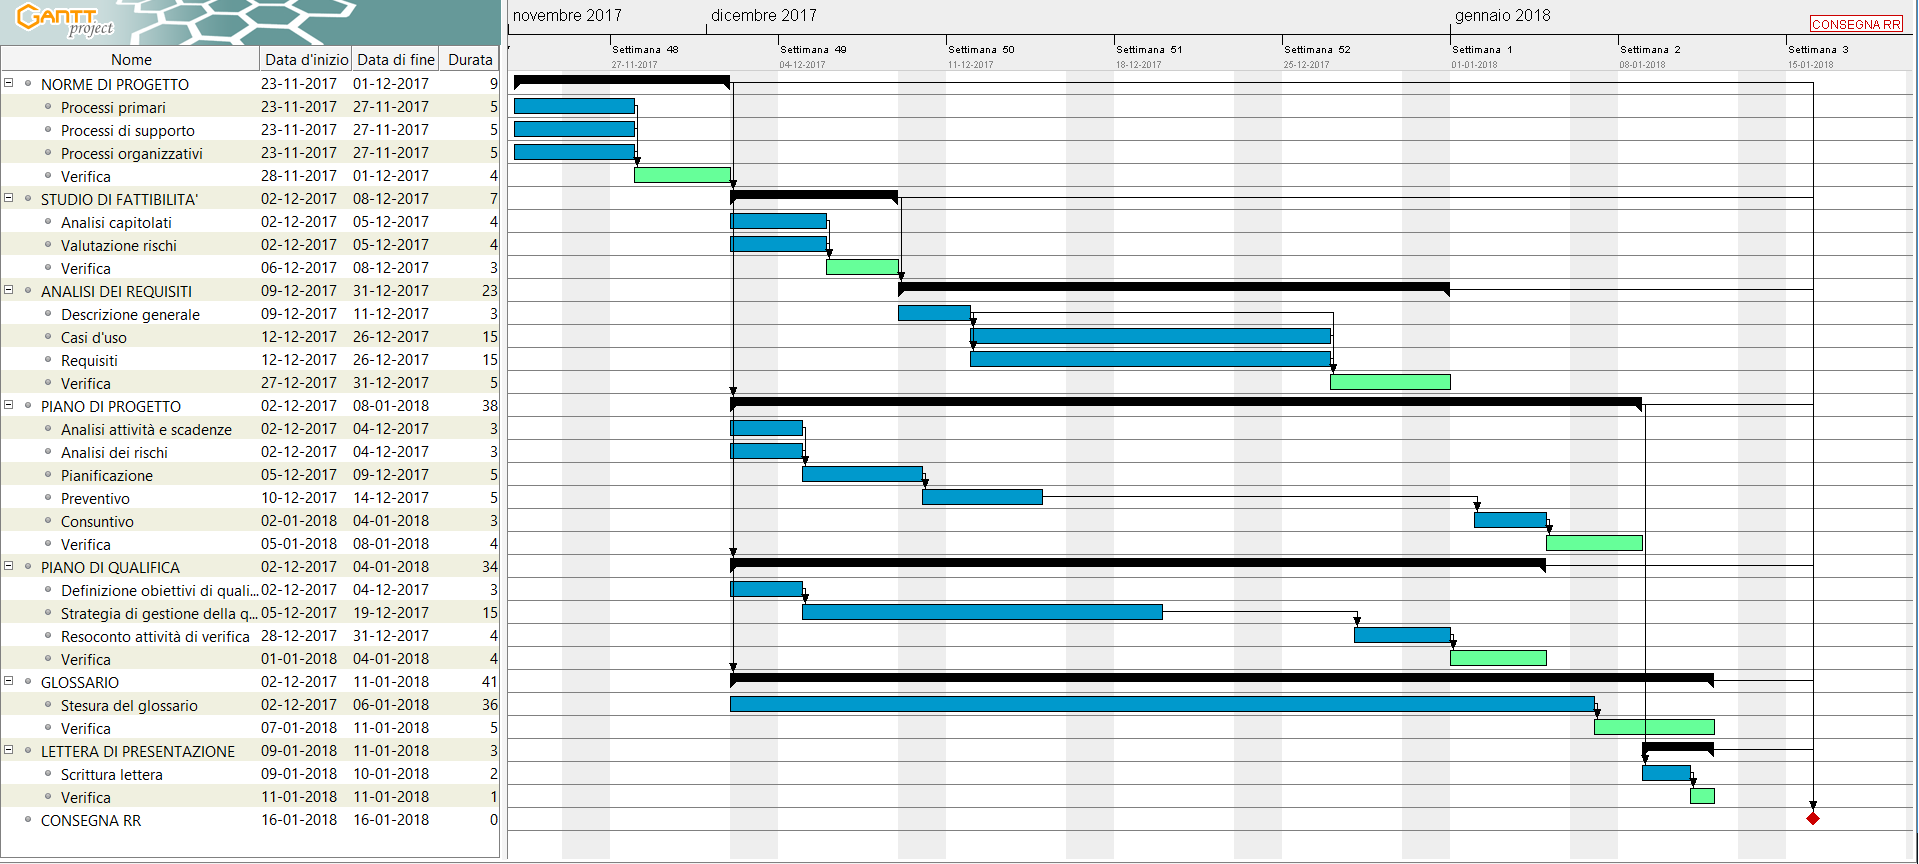
\includegraphics[width=20.5cm]{images/gantt/analisi.png}
		\label{fig:foo}
		\caption{Diagramma di Gantt del periodo di Analisi}		
	\end{figure}			
\end{landscape}	

\section{Consolidamento dei requisiti}
\subsection{Consolidamento dei requisiti - Diagramma di Gantt}

\section{Progettazione architetturale}
\subsection{Progettazione architetturale - Diagramma di Gantt}

\section{Progettazione di dettaglio e codifica}
\subsection{Progettazione di dettaglio e codifica - Diagramma di Gantt}

\section{Validazione e collaudo}
\subsection{Validazione e collaudo - Diagramma di Gantt}

\end{document}